\documentclass[aps,prl,superscriptaddress,groupedaddress]{revtex4}
\usepackage{graphicx}  % needed for figures
\usepackage{dcolumn}   % needed for some tables
\usepackage{bm}        % for math
\usepackage{amssymb,amsmath} % for math
\usepackage{tikz} % for drawing
\usepackage{subfig} % for subfigure
\usetikzlibrary{calc} % for tikz calculations
\usetikzlibrary{arrows,decorations.markings} % make arrow head bigger
\usepackage{array} % for changing table height
\usepackage{comment}
\usepackage[bookmarks]{hyperref}
%\usepackage{siunitx} % for decimal alignment in tables
%\usepackage{arydshln} % for dashed line in tables

% avoids incorrect hyphenation, added Nov/08 by SSR
\hyphenation{ALPGEN}
\hyphenation{EVTGEN}
\hyphenation{PYTHIA}

\begin{document}

\widetext
\title{Accurate Predictions of Ionization and Atomization Energies without the Born-Oppenheimer Approximation}
\author{Yubo Yang}
\author{Ilkka Kyl\"{a}np\"{a}\"{a}}
\author{Norm M. Tubman}
\affiliation{Department of Physics, University of Illinois, Urbana, Illinois 61801 USA}
\author{Jaron T. Krogel}
\affiliation{Materials Science \& Technology Division, Oak Ridge National Laboratory, Oak Ridge, TN 37831}
\author{Sharon Hammes-Schiffer}
\affiliation{Department of Chemistry, University of Illinois, Urbana, Illinois 61801 USA}
\author{David M. Ceperley}
\affiliation{Department of Physics, University of Illinois, Urbana, Illinois 61801 USA}
\date{\today}

\begin{abstract}
We obtained ground-state energies of a range of small atoms and molecules with Fixed-Node Diffusion Monte Carlo (FN-DMC) to an accuracy of $0.01\text{mHa}$ ($0.27\text{meV}$), treating both electrons and ions as quantum particles. We used "dragged node approximation" developed by Tubman et. al to construct the trial wavefunction without the adiabatic assumption. For each system, we optimized an all-electron trial wavefunction generated by quantum chemistry methods and used it to construct an all-electron-ion wavefunction. It is then used in FN-DMC to obtain the ground-state energy of said system. We found the ionization energies of first row atoms to be identical with or without the adiabatic assumption, whereas the atomization energies of simple hydrides to change by as much as 6.2\%. The non-adiabatic results are in better agreement with the best available quantum chemistry literature in all tested hydrides.
\end{abstract}
\maketitle

\section{Introduction}
The Born-Oppenheimer Approximation\cite{BO} allows the separation of time scales of the electron and ion problems and greatly reduces the complexity of the Hamiltonian to be solved. It is such a good approximation that it is inherently adopted in much of the \textit{Ab initio} studies. However, there are cases where the Born-Oppenheimer approximation fails, that is when the coupling between the electron and nuclei motions become important, especially in the presence of light nuclei. It has been shown that the inclusion of non-adiabatic effects is crucial for accurately characterizing the stability of atomic hydrogen as well as predicting its ground state crystal structure \cite{Ceperley_1987,Natoli_1993,Natoli_1995}. The coupling between electron and nuclei motions is also important in distinguishing the hydrogen atom transfer (HAT) and proton-coupled electron transfer (PCET) mechanisms \cite{Sirjoosingh_PCET}. Current efforts in incorporating  non-adiabatic effects are often costly either in human time or computational time. We would like to demonstrate that with minimum modification to the existing fixed-node diffusion Monte Carlo (FN-DMC), one can obtain highly accurate results without the Born-Oppenheimer approximation.

Studies that include non-adiabatic effects are scarce. Here we note two approaches that offer similar or better accuracy than our method. The first approach is to add corrections to a basic coupled cluster calculation \cite{Feller_Corrections}. In such an approach, a frozen-core coupled cluster singles and doubles (FC-CCSD) \cite{Purvis_CCSD} calculation serves as a first approximation for the ground-state energies. Then a series of corrections including core/valance, spin-orbit coupling, higher order correlation, zero point motion, diagonal Born-Oppenheimer and scalar relativistic effects are introduced. This method produces highly accurate expectation values, but contains uncontrolled errors that have to be estimated either empirically or analyzed on a molecule-by-molecule basis \cite{Feller_Error}. Another approach in a more recent development is to use the explicitly correlated Gaussian (ECG) basis \cite{Adamowicz_ECG,Mitroy_ECG}. This approach is capable of calculating the ground-state energies of small molecules to an incredibly high accuracy. Unfortunately, the current implementation of ECG cannot be applied to moderately-sized systems due to factorial scaling in computational cost with the number of identical particles \cite{Bubin_BH_noBO}. Other methods with less aggressive scaling include nuclear-electronic orbital (NEO) Hatree-Fock (HF) \cite{Sharon_NEO}, NEO explicitly correlated HF (NEO-ECHF) \cite{Sharon_NEOX,Sharon_NEOX1,Sharon_NEOX2}, path integral Monte Carlo \cite{Ilkka_Path,Ilkka_Path1,Ilkka_Path2} and multicomponent density functional theory \cite{Sharon_NEO-DFT,Sharon_NEO-DFT1,Sharon_NEO-DFT2,Sharon_NEO-DFT3,Gross_NEO-DFT,Gross_NEO-DFT1}. While these methods can be applied to larger systems, it would be difficult to deliver the same kind of accuracy that ECG offers without significant development.

We acknowledge the subtle difference between the Born-Oppenheimer approximation and the adiabatic assumption, namely the former includes the kinetic energy of nuclei on a single electronic potential surface whereas the latter doesn't \cite{Cederbaum_BO}. Here we will only consider the adiabatic limit, where the ions are "clamped" and their kinetic energies ignored and the fully non-adiabatic case, where the exact non-relativistic Hamiltonian is used. One might equivalently refer to the latter as non-Born-Oppenheimer. We do not consider spin-orbit coupling effects in either case.

\section{Method}

\subsection{Fixed-Node Diffusion Monte Carlo (FN-DMC)}
Diffusion Monte Carlo is a projector method that evolves a trial wavefunction with the exact Hamiltonian in imaginary time and projects out the ground-state wavefunction in the infinite time limit. The trial wavefunction is often produced by some other mean field method such as Hartree-Fock (HF) or Density Functional Theory (DFT). The more popular variant (FN-DMC) introduces the fixed-node approximation to overcome the sign-problem suffered in fermion problems due to the presence of nodes in the ground-state wavefunction. FN-DMC is a simple but powerful method, since its accuracy is only limited by the quality of the nodal surface of the trial wavefunction and the finite length of the calculation. The uncertainty in the obtained ground-state energy is statistically controlled and may be shrunk arbitrarily by increasing computation time. If the trial wavefunction has the same nodal surface as the exact ground-state wavefunction, the final ground-state energy will be exact with zero variance. It should be noted that even with an approximate nodal surface, FN-DMC will still produce an excellent approximation of the exact ground-state energy, albeit with rather large variance if the quality of the trial function is low. In addition, since the exact Hamiltonian is used, the FN-DMC method is variational, that is, even when the nodes of the trial wavefunction are not exact the result will be a rigorous upper bound to the exact ground-state energy.

Due to the introduction of linear optimization method by Nightingale et. al.\cite{Nightingale_Linear} and Umrigar et. al.\cite{Umrigar_Linear}, one can systematically improve the wave function ansatz generated by quantum chemistry calculations to obtain high quality wave functions for atoms and molecules as was done by Brown\cite{Brown_Bench} and Toulouse\cite{Toulouse_Bench}. However, in these benchmark studies, the authors always worked within the adiabatic assumption, i.e. only the electron Hamiltonian is used in evolving the trial wavefunction in imaginary time, while the ions are "clamped" to their equilibrium positions. Such an assumption is not fundamentally required by FN-DMC. It's inclusion is mostly due to a lack of mean field theories that include non-adiabatic effects. Although there is significant effort in the quantum chemistry community to develop such methodology as mentioned in the introduction, until a standardized package is developed we will have to rely on modification of the QMC algorithm itself to include non-adiabatic effects. To this end, we will use the technique developed by Tubman et. al. \cite{Tubman_ECG} to construct a high quality all-electron-ion wavefunction from an optimized all-electron wavefunction.

\subsection{Electron Wavefunction and Optimization}
We followed the basic strategies of Umrigar et. al.\cite{Umrigar_Alleviation,Toulouse_Bench} and Needs et. al. \cite{Brown_Bench,Seth_Bench} in generating our all-electron wavefunctions. The initial guess for the wavefunction is generated from Complete Active Space Self-Consistent Field (CASSCF) \cite{Chaban_MCSCF,Szabo} calculation using the quantum chemistry package GAMESS-US\cite{GAMESS}. The optimized orbitals are then used in a Second Order Configuration Interaction (SOCI) calculation to generate a series of Configuration State Functions (CSF). This process is described in more detail in \cite{Clark_Bench}. The multi-CSF expansion of the wavefunction generated by GAMESS can be expressed in the following form
\begin{align}
\Psi_{SOCI}(\vec{r})=\sum\limits_{i=1}^{N_{CSF}}\alpha_i\phi_i(\vec{r}) \label{eq:psi_gms}
\end{align}
where $\vec{r}$ refers to the spacial coordinates of all the electrons. $\phi_i(\vec{r})$ are the CSF generated from SOCI. We used the cc-pV5Z basis for all the atomic systems but switched to Roos Augmented Triple Zeta ANO basis for molecular systems due to GAMESS's limited ability to handle a large number of basis elements. Both basis sets are taken from Basis Set Exchange \cite{BSE}.

A Jastrow factor $J(\vec{r},\vec{\beta})$, in the form of a B-spline with values $\vec{\beta}$ on a linear grid, is then added to the wave function to correlate electron motion and smooth out the divergence in the local energy near the ions by imposing the cusp condition \cite{Kato}. Our Jastrow factor contains one electron-ion term, two electron-electron terms (one for same spin electrons, one for opposite spin electrons) and two electron-electron-ion terms. The actually wave function being optimized is then
\begin{align}
\Psi_e(\vec{r})=e^{J(\vec{r},\vec{\beta})}\sum\limits_{i=1}^{N_{CSF}}\alpha_i\phi_i(\vec{r})\label{eq:psie}
\end{align}
We optimized the CSF and Jastrow coefficients $\vec{\alpha},\vec{\beta}$ simultaneously with QMCPACK\cite{QMCPACK}.

\subsection{Electron-Ion Wavefunction}

\begin{figure*}[hpb]
\centering
\subfloat[][Hydrogen atom]{\documentclass{standalone}
\usepackage{tikz}
\usetikzlibrary{calc} % for tikz calculations
\usetikzlibrary{arrows,decorations.markings} % make arrow head bigger

% set up externalization
\usetikzlibrary{external}
\tikzset{external/system call={latex \tikzexternalcheckshellescape -halt-on-error
-interaction=batchmode -jobname "\image" "\texsource" && 
dvips -o "\image".ps "\image".dvi &&
ps2eps "\image.ps"}}
\tikzexternalize[shell escape=-enable-write18] % MikTeX uses a -enable-write18 instead of --shell-escape.
% compile with: latex -enable-write18

\begin{document}

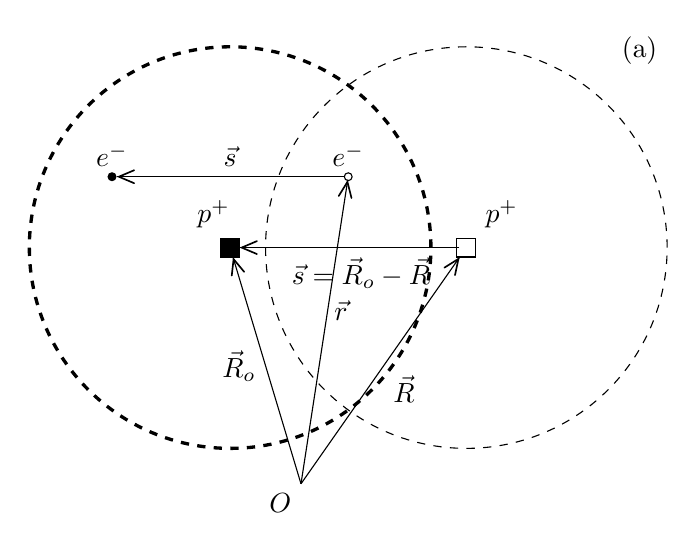
\begin{tikzpicture}
% define arrow head
[
    decoration={
      markings,
      mark=at position 1 with {\arrow[scale=1.5,black]{angle 45}};
    }
]

% scale
\pgfmathsetmacro{\a}{3}
\coordinate (H1) at (0,0);
\coordinate (H) at (\a,0);

% coordinate
\coordinate (O) at ($0.5*(H1)+0.3*(H)-(0,\a)$);
\node at (O) [below left]{$O$};

% ions
\pgfmathsetmacro{\R}{0.04*\a} % ion radius
\draw[fill] ($(H1)-(\R,\R)$) rectangle ($(H1)+(\R,\R)$) node [above left] {$p^+$};
\draw ($(H)-(\R,\R)$) rectangle ($(H)+(\R,\R)$) node [above right] {$p^+$};
\draw[postaction={decorate}] (O) -- ($0.96*(H)+0.04*(O)$);
\node at ($0.5*(H)+0.5*(O)$) [below right] {$\vec{R}$};
\draw[postaction={decorate}] (O) -- ($0.96*(H1)+0.04*(O)$);
\node at ($0.5*(H1)+0.5*(O)$) [left] {$\vec{R}_o$};

% wave function contour
\draw[very thick,dashed] (H1) circle (0.85*\a);
\draw[dashed] (H) circle (0.85*\a);

\coordinate (e) at (.5*\a,.3*\a);
\coordinate (e1) at ($(e)-(H)$);

% electrons
\node[draw,circle,inner sep=1pt] at (e) {};
\node at (e) [above] {$e^-$};
\node[draw,circle,inner sep=1pt,fill] at (e1) {};
\node at (e1) [above] {$e^-$};

% vectors
\draw[postaction={decorate}] (O) -- ($0.99*(e)+0.01*(O)$);
\node at ($0.5*(e)+0.5*(O)$) [above right] {$\vec{r}$};
\draw[postaction={decorate}] ($0.97*(H)$)--($0.04*(H)$);
\node at ($0.5*(H1)+0.22*(H)$) [below right] {$\vec{s}=\vec{R}_o-\vec{R}$};

\draw[postaction={decorate}] ($(e)-(0.02*\a,0)$) -- ($(e1)+(0.02*\a,0)$);
\node at ($0.5*(e)+0.5*(e1)$) [above] {$\vec{s}$};
%\draw[postaction={decorate}] (O) -- ($0.99*(e1)+0.01*(O)$);
%\node at ($0.5*(O)+0.5*(e1)$) [below left] {$\vec{r'}$};

% subplot marking
\node at (5.2,2.5) {(a)};

\end{tikzpicture}

\end{document}}
\subfloat[][$H_2^+$ molecule]{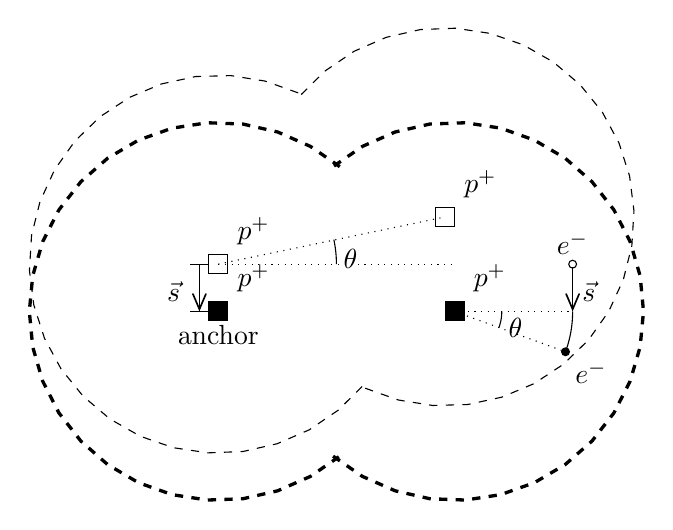
\begin{tikzpicture}
% define arrow head
[
    decoration={
      markings,
      mark=at position 1 with {\arrow[scale=1.5,black]{angle 45}};
    }
]
% scale
\pgfmathsetmacro{\a}{3}
\coordinate (H1) at (0,0);
\coordinate (H) at (\a,0);

% ions
\pgfmathsetmacro{\R}{0.04*\a} % ion radius
\draw[fill] ($(H1)-(\R,\R)$) rectangle ($(H1)+(\R,\R)$) node [above right] {$p^+$};
\draw[fill] ($(H)-(\R,\R)$) rectangle ($(H)+(\R,\R)$) node [above right] {$p^+$};
\draw [domain=50:310,dashed,very thick] plot ({0.8*\a*cos(\x)}, {0.8*\a*sin(\x)});
\draw [domain=-130:130,dashed,very thick] plot ({0.8*\a*cos(\x)+\a}, {0.8*\a*sin(\x)});
\node at ($(H1)-(0,0.1*\a)$) {anchor};

\pgfmathsetmacro{\s}{0.2*\a}
\draw[postaction={decorate}] ($(H1)+(-2*\R,\s)$) -- ($(H1)+(-2*\R,0)$);
\draw  ($(H1)+(-\R,\s)$) -- ($(H1)+(-3*\R,\s)$);
\draw  ($(H1)+(-\R,0)$) -- ($(H1)+(-3*\R,0)$) node [above left] {$\vec{s}$};
\coordinate (H1) at (0,\s);
\coordinate (H) at ($(\a-0.2*\s,2*\s)$);
% ions
\draw ($(H1)-(\R,\R)$) rectangle ($(H1)+(\R,\R)$) node [above right] {$p^+$};
\draw ($(H)-(\R,\R)$) rectangle ($(H)+(\R,\R)$) node [above right] {$p^+$};
\draw [domain=65:320,dashed] plot ({0.8*\a*cos(\x)}, {0.8*\a*sin(\x)+\s});
\draw [domain=-115:140,dashed] plot ({0.8*\a*cos(\x)+\a-0.2*\s}, {0.8*\a*sin(\x)+2*\s});

% electrons
\coordinate (e) at (1.5*\a,\s);
\node[draw,circle,inner sep=1pt] at (e) {};
\node at (e) [above] {$e^-$};
\draw[postaction={decorate}] ($(e)-(0,0.07*\s)$) -> ($(e)-(0,\s)$) node [above right] {$\vec{s}$};
\pgfmathsetmacro{\t}{20} % angle of electron
\coordinate (e1) at ({0.5*\a*cos(-\t)+\a}, {0.5*\a*sin(-\t)});
\draw [domain=0:-\t] plot ({0.5*\a*cos(\x)+\a}, {0.5*\a*sin(\x)});
\node[draw,circle,inner sep=1pt,fill] at (e1) {};
\node at (e1) [below right] {$e^-$};

% angle
\draw[dotted] (H1) -- (\a,\s); 
\draw[dotted] (H1) -- (H); 
\draw[dotted] (\a,0) -- ($(e)-(0,\s)$); 
\draw[dotted] (\a,0) -- ($(e1)$);
\draw[domain=0:12] plot ({0.5*\a*cos(\x)}, {0.5*\a*sin(\x)+\s}) node [below right] {$\theta$};
\draw[domain=0:-20] plot ({0.2*\a*cos(\x)+\a}, {0.2*\a*sin(\x)}) node [right] {$\theta$};
\end{tikzpicture}}
\caption{\textbf{Dragged Node Approximation} (a) For hydrogen atom, we assume the entire wavefunction shifts with the ion. This process can be visualized by following a contour of the wavefunction. The thick dashed circle represents a contour of the electron wavefunction when the proton is at its reference position $\vec{R}_o$ and the thin dashed circle represents the same contour when the proton has moved to a new position $\vec{R}$. To evaluate the ion-dependent electron wavefunction $\bar{\psi}_e(\vec{r},\vec{R})$, we simply map the electron to its proper place in the reference wavefunction $\psi_e(\vec{r})$. That is $\bar{\psi}_e(\vec{r},\vec{R})=\bar{\psi}_e(\vec{r}+\vec{s},\vec{R}_o)=\psi_e(\vec{r}+\vec{s})$ where $\vec{s}$ is the shift required to put the the proton back to its reference position. (b) For $H_2^+$, we pick one of the protons as an "anchor" and approximate the new wavefunction by dragging the reference wavefunction with the "anchor" proton. We also rotate the wavefunction to align its axis of symmetry with the orientation of the two protons. \label{fig:drag} }
\end{figure*}

Once a satisfactory electron wave function has been obtained, we construct the electron-ion wave function using the following ansatz suggested by Tubman et. al.\cite{Tubman_ECG}
\begin{align}
\Psi_{ei}(\vec{r},\vec{R})=\psi_I(\vec{R})\bar{\psi}_e(\vec{r},\vec{R}) \label{eq:psi}
\end{align}
where $\vec{R}$ includes spatial coordinates of all ions. The ion wave function consists of simple products of Gaussian wave functions over each nuclei pair.
\begin{align}
\psi_I(\vec{R})\propto \prod\limits_{i,i<j}e^{-a(\vert \vec{R}-\vec{R}_j\vert-b_{ij})^2}
\end{align}
where $a$ is a contraction coefficient for the ion wave function that we optimize for each system and $b_{ij}$ are taken to be the equilibrium distances between the nuclei in the adiabatic limit. Notice the new electron wavefunction $\bar{\psi}_e$ depends on both the electron and the ion positions. In general $\bar{\psi}_e(\vec{r},\vec{R})\neq\psi_e(\vec{r})$, but we do have $\bar{\psi}_e(\vec{r},\vec{R}_o)=\psi_e(\vec{r})$, where $\vec{R}_o$ are the ion positions used in the creation of the $\psi_e(\vec{r})$. The most straight-forward way to obtain $\bar{\psi}(\vec{r},\vec{R})$ is to repeat the process described in the previous section for every new ion positions $\vec{R}$. However, such an approach would be horrendously expensive. To alleviate the computational cost, Tubman et. al. proposed a "Dragged Node Approximation" \cite{Tubman_ECG}, where the contours (including the nodal surface) of $\psi_e(\vec{r})$ are dragged along the ions $\vec{R}$ to create $\bar{\psi}(\vec{r})$. Figure \ref{fig:drag} demonstrates this strategy for the simple cases of a hydrogen atom and a $H_2^+$ molecule. For atoms, this "dragged-node" process is equivalent to re-running a quantum chemistry calculation and re-optimizing the wavefunction at each new ion position. However, for diatomic molecules, since the distance between ions fluctuates, the two processes will produce slightly different wavefunctions. It is also important to note that the trial wavefunction (\ref{eq:psi}) is still in Born-Oppenheimer form for each set of ion coordinates, that is we are essentially using the Born-Oppenheimer wavefunction as the starting point of FN-QMC. Nevertheless, without modification to the Hamiltonian, FN-DMC will automatically include non-adiabatic effects not present in the trial wavefunction and the process remains variational.

Although the dragged-node technique is developed with atomic and diatomic systems in mind, it is not difficult to generalize it for use in larger systems or even apply to parts of a bigger system, treating light ions as quantum particles and heavy ions as "clamped". For a system of more than 3 particles, a general fitting procedure \cite{Kabsch_Rotation} can be done to determine the transformation needed to put the ions back to their reference positions. This is similar to the process of protein structure alignment implemented in some well-known biophysics software such as VMD \cite{VMD}. Once the transformation is determined, we can map each electron individually and evaluate the wavefunction with moved ions using the reference wavefunction as was done for atoms and diatomics. One complication occurs when the ions become degenerate (when there are more than two protons with the same spin for example). In this case one has to explicitly anti-symmetrize the ion wavefunction in a manner similar to what's done for the electron wavefunction (Slater determinant). 

\section{Results and Discussion}

\subsection{Ground State Energies}

Ground state energies were calculated for first row atoms and ions with and without the adiabatic assumption (Table \ref{tab:ionization}). The first row of Table \ref{tab:ionization} lists the level of CASSCF calculation we used to generate the all-electron wavefunction guess. We first performed a CAS(m,n) calculation, meaning that we distribute of m electrons into n active orbitals, with the ground-state equilibrium geometries taken from experimental data\cite{CCCBDB}. The MCSCF optimized orbitals are then used in a SOCI calculation that includes single and double excitations of the m electrons into all of the available valance orbitals provided by the basis. The SOCI ground state CSF $\phi_0(\vec{r})$ always dominates the expansion (with $\alpha_0>.95$). Nevertheless, we include all CSFs with coefficients bigger than some cutoff $\epsilon$ to lend reasonable flexibility to the wavefunction during optimization. The choice of $\epsilon$ is somewhat arbitrary. We wish to included as many CSFs as possible to maximize the flexibility of the wavefunction. However, the inclusion of too many CSFs with small expansion coefficients introduces unnecessary noise into the system and requires a large number of samples in the optimization step to reach our desired accuracy. Therefore, we have chosen $\epsilon$ to restrict the number of CSFs in the wave function to be $\sim$1000 in all systems to maintain a balance between the flexibility and the cost of optimization. In all of the atoms and molecules tested, this criteria results in an $\epsilon$ of $0.001\sim0.0001$ and the sum of coefficients squared of the included CSFs $\sum a_i^2 > 0.999$ in all cases. Optimization was performed with $6\times10^6$ statistically independent samples and we chose a cost function consisting of equal parts average local energy and reweighted variance. We found this choice of cost function to produce slightly better wavefunctions than a highly biased one, albeit the differences are small and are most likely insignificant at the DMC level. 

We also performed timestep extrapolation for all of the tested systems. Five timesteps from $0.005\text{Ha}^{-1}$ to $0.001\text{Ha}^{-1}$ were used for all systems in the adiabatic FN-DMC. A smaller timestep ($0.0005\text{Ha}^{-1}$) is used for systems with 7 or more electrons. For such small timesteps almost all DMC runs have $>99\%$ acceptance rate, thus we expect the timestep error to be very small. Indeed, for systems with fewer than 7 electrons, the DMC energies at all tested timesteps agree within error bars, only larger systems exhibit linear extrapolation behavior.

The adiabatic ground state energies of atoms are in perfect agreement with the most recent QMC benchmark study \cite{Seth_Bench}. The non-adiabatic ground-state energies for Be and B ($-14.66643(2)$Ha and $-24.65244(3)$Ha) are in good agreement with ECG results ( -$14.66643544$Ha \cite{Bubin_BeH_noBO} and -$24.652598$Ha\cite{Bubin_BH_noBO}). Even though we used massive multi-determinant expansions ($\sim$ 1000 CSF) in our study whereas Seth et. al. \cite{Seth_Bench} used moderately-sized multi-determinant expansions ($\sim$ 100 CSF) with a backflow transformation. We obtained almost the same DMC energies with very different wavefunctions.

Similar calculations were performed for diatomic systems (Table \ref{tab:atomization}) and the results are in excellent agreement with the sophisticated coupled cluster study \cite{Feller_Corrections}. It is important to note that with our method, the only included non-adiabatic effects are the zero point motion of the nuclei and any correlation that may exist among the quantum particles. We do not take into account spin-orbit coupling or relativistic effects. Therefore, we subtracted the corresponding corrections in \cite{Feller_Corrections} for a fair comparison. Specifically, we took the reference energies from the last column of Table VI of \cite{Feller_Corrections} and subtracted off the corrections in the $\Delta E_{SR}$ and SO columns for comparison with our non-adiabatic energies and further subtracted off the DBOC and ZPE correction for comparison with our adiabatic energies.

However, our method is much simpler. There's no need for separate computation for each correction factor, thus no addition of uncertainties. Further, the uncertainties in our calculations are statistically controlled and may be reduced by increasing computation time. 

\subsection{Ionization Energies}
The ionization energies are listed at the end of Table \ref{tab:ionization} and they agree well with experimental results. Notice that even though ground state energies change significantly with the inclusion of non-adiabatic effects, the ionization energies match perfectly with or without the adiabatic assumption. This suggests that for atomic systems, the gradient coupling between electron and ion motions is indeed negligible. The difference in ground state energies can be entirely attributed to the zero point motion of the nuclei. Physically, this means that for all first row atoms, the outer most electron is perfectly screened from the nucleus and all of the energy required for its removal can be attributed to its interaction with the rest of the electrons in the atom.

The ground state energy of $\text{LiH}^-$ was also calculated to obtain the electron affinity of LiH. The energy obtained in the adiabatic limit at the DMC level is $-8.08220(2)$Ha and $-8.07811(3)$Ha with non-adiabatic effects included. Our non-adiabatic result is in good agreement with a previous ECG study \cite{Bubin_LiH_noBO} which reported a value of $-8.07856887$Ha. We report an electron affinity of $0.01191(4)$Ha which is very close to the ECG prediction of $0.012132(2)$Ha and agrees with experiment $0.0126(4)$Ha up to the mHa level. It should be noted that the authors of \cite{Bubin_LiH_noBO} mislabeled the columns for ground state energies of $\text{LiH}^-$ and LiD resulting in a miss-citation in \cite{Mitroy_ECG}.

\begin{table*}[htpb!]
\setlength{\extrarowheight}{3pt}
\begin{tabular}{*{1}{*{8}{c}}}
\hline\hline
$\text{Atom}$ & $\text{Li}(^2\text{S)}$ & $\text{Be}(^1\text{S)}$ & $\text{B}(^2\text{P)}$ & $\text{C}(^3\text{P)}$ & $\text{N}(^4\text{S)}$ & $\text{O}(^3\text{P)}$ & $\text{F}(^2\text{P)}$ \\ \hline
This Work & $\text{-7.478056(4)}$ & $\text{-14.66732(1)}$ & $\text{-24.65377(1)}$ & $\text{-37.84449(2)}$ & $\text{-54.58858(3)}$ & $\text{-75.06576(4)}$ & $\text{-99.7316(1)}$ \\
Seth 2011 \cite{Seth_Bench} & $\text{-7.478067(5)}$ & $\text{-14.667306(7)}$ & $\text{-24.65379(3)}$ & $\text{-37.84446(6)}$ & $\text{-54.58867(8)}$ & $\text{-75.0654(1)}$ & $\text{-99.7318(1)}$ \\
Davidson 1993 \cite{Davidson_Atoms} &  -7.47807 & -14.66736 & -24.65391 & -37.8450 &-54.5892 & -75.0673 & -99.7339 \\
This Work (full) & $\text{-7.47742(1)}$ & $\text{-14.66643(2)}$ & $\text{-24.65244(3)}$ & $\text{-37.84277(6)}$ & $\text{-54.58655(8)}$ & $\text{-75.0631(1)}$ & $\text{-99.7290(4)}$ \\
\hline
\end{tabular} \\ 
\begin{tabular}{*{1}{*{8}{c}}}
$\text{Ion}$ & $\text{Li}^+(^1\text{S)}$ & $\text{Be}^+(^2\text{S)}$ & $\text{B}^+(^1\text{S)}$ & $\text{C}^+(^2\text{P)}$ & $\text{N}^+(^3\text{P)}$ & $\text{O}^+(^4\text{S)}$ & $\text{F}^+(^3\text{P)}$ \\ \hline
This Work & $-7.279919(4)$ & $\text{-14.324753(6)}$ & $\text{-24.34884(1)}$ & $\text{-37.43075(2)}$ & $\text{-54.05376(3)}$ & $\text{-74.56588(4)}$ & $\text{-99.0913(1)}$ \\
Seth 2011 \cite{Seth_Bench} & $\text{-7.279914(3)}$ & $\text{-14.324761(3)}$ & $\text{-24.34887(2)}$ & $\text{-37.43073(4)}$ & $\text{-54.05383(7)}$ & $\text{-74.56662(7)}$ & $\text{-99.0911(2)}$ \\
Davidson 1993 \footnotemark[1] \cite{Davidson_Atoms} & -7.27999 & -14.3249 & -24.3489 & -37.4312 & -54.0552 & -74.5668 & -99.0937 \\
This Work (full) & $\text{-7.2793(1)}$ & $\text{-14.32386(2)}$ & $\text{-24.34750(3)}$ & $\text{-37.42904(4)}$ & $\text{-54.05182(9)}$ & $\text{-74.56336(8)}$ & $\text{-99.0885(3)}$ \\
\hline
IP & 0.19814(1) & 0.34256(2) & 0.3049(3) & 0.4138(5) & 0.53475(8) & 0.500(1) & 0.640(1) \\
IP (full) & 0.1981(1) & 0.34257(2) & 0.3049(3) & 0.4137(5) & 0.53473(8) & 0.500(1) & 0.640(1) \\
Exp. \cite{Davidson_Atoms} & 0.19808 & 0.3425 & 0.30502 & 0.413797 & 0.533967 & 0.500526 & 0.640173 \\
\hline
\end{tabular}
\footnotetext[1]{The ionic ground state energies are calculated by adding ionization potentials in Table XII to the atomic ground state energies in Table XI from \cite{Davidson_Atoms} }
\caption{\textbf{Ionization Energies} Fixed-Node DMC was performed with and without the adiabatic assumption and the energies for each atom and ion is reported in units of Hartree. The label (full) means we treat both electrons and ions quantum mechanically. \label{tab:ionization}}
\end{table*}
 
\subsection{Atomization Energies}
The ground state energies of first row hydrides are reported in Table \ref{tab:atomization}. The energies calculated in the adiabatic limit are on par and sometimes better than the best available quantum chemistry results \cite{Adamowicz_LiH,Koput_BeH,Miliordos_BH} and the energies calculated without the adiabatic assumption are in excellent agreement with state-of-the-art quantum chemistry calculations performed with ECG where available (LiH,BeH and BH). In the case of simple hydrides, non-adiabatic effects do make a noticeable contribution to the atomization energy. This is possibly due to the presence of the light weighted proton.
 
\begin{table}[htpb!]
\setlength{\extrarowheight}{3pt}
\begin{tabular}{*{1}{*{7}{c}}}
\hline\hline
$\text{Molecule}$ & $\text{LiH }(^1\Sigma^+)$ & $\text{BeH }(^2\Sigma^+)$ & $\text{BH }(^1\Sigma^+)$ & $\text{CH }(^2\Pi)$ & $\text{OH }(^2\Pi)$ & $\text{HF }(^1\Sigma^+)$ \\ \hline
This Work & $\text{-8.070521(7)}$ & $\text{-15.24793(1)}$ & $\text{-25.28868(2)}$ & $\text{-38.4781(1)}$ & $\text{-75.7352(1)}$ & $\text{-100.44941(6)}$ \\
$E_{\text{ref}}$ \footnotemark[1] \cite{Adamowicz_LiH,Koput_BeH,Miliordos_BH,Davidson_Atoms,Feller_Corrections} & $\text{-8.07045}$ & $\text{-15.247846}$ & $\text{-25.287650}$ & $\text{-38.4792(2)}$ & $\text{-75.7382(2)}$ & $\text{-100.4600(3)}$ \\
This Work (full) & $\text{-8.06620(2)}$ & $\text{-15.24196(7)}$ & $\text{-25.28103(4)}$ & $\text{-38.4704(4)}$ & $\text{-75.7260(4)}$ & $\text{-100.4391(4)}$ \\
ECG \cite{Bubin_LiH_noBO,Bubin_BeH_noBO,Bubin_BH_noBO} & $\text{-8.0664371(15)}$ & $\text{15.24203(10)}$ & $\text{-25.2803(10)}$ & $\text{N/A}$ & $\text{N/A}$ & $\text{N/A}$ \\
\hline
$D_{e}$ & 0.092465(8) & 0.08062(1) & 0.13491(2) & 0.13361(2) & 0.16944(4) & 0.21781(6) \\
Feller 2008\footnotemark[2] \cite{Feller_Corrections} & 0.09262(5) & 0.0809(4) & 0.1354(2) & 0.1342(2) & 0.1709(2) & 0.2258(3) \\
$D_{e}$ (full) & 0.08905(2)  & 0.07580(7)  & 0.12886(5) & 0.1279(7) & 0.16317(4) & 0.21037(5) \\
Feller 2008\footnotemark[3] \cite{Feller_Corrections} & 0.08940(5) & 0.0761(4) & 0.1299(2) & 0.1276(2) & 0.1622(2) & 0.2166(3)\\
Exp. \cite{CCCBDB} & 0.08874(38) & 0.0826(11) & 0.1281(37) & 0.1275(5) & 0.1622(1) & 0.2158(3) \\
\hline\hline
\end{tabular}
\footnotetext[1]{For the smaller systems (LiH, BeH and BH), ECG studies provide the best reference energies. For CH, OH and HF, we combined the atomic energies in \cite{Davidson_Atoms} with the atomization energies in \cite{Feller_Corrections} to produce the reference energies. }
\footnotetext[2]{The non-relativistic atomization energy in the adiabatic limit are calculated by subtracting the scalar relativistic, spin-orbit coupling and zero-point energy corrections from the reference energies in Table VI of \cite{Feller_Corrections} }
\footnotetext[3]{Here only the scalar relativistic and spin-orbit coupling corrections are subtracted}
\caption{\textbf{Atomization Energies} Fixed-Node DMC was performed with and without the adiabatic assumption for all first row hydrides. All energies are reported in units of Hartree. The label (full) means we treat both electrons and ions quantum mechanically.\label{tab:atomization}}
\end{table} 

\section{Conclusion}
We calculated the ground-state energies of first row atoms and their corresponding ions and hydrides to an accuracy of $0.1$mHa both with and without the adiabatic assumption. We found the ionization energies of the atoms to be independent of the adiabatic assumption, suggesting that either the energy difference between the adiabatic and non-adiabatic ground states is entirely due to the zero point motion of the nuclei or the coupling between the nucleus and electrons is not important in the ionization process. The atomization energies of simple hydrides were significantly different in the adiabatic than in the non-adiabatic limit, possibly due to the presence of a light nucleus (the proton) in the molecule. We showed that it is necessary to include non-adiabatic effects to accurately predict the experimental values of atomization energies for these simple hydrides.

These calculations also verified the validity of the "dragged-node" approximation, namely it does indeed produce a high quality electron-ion trial wavefunction from a good electron wavefunction. This technique also has the potential to solve more interesting problems due to its ease of implementation as well as the polynomial scaling in computational time with respect to the number of electrons. As mentioned at end of Method section, this technique can be generalized quite easily to deal with larger systems. In addition, we are able to offer similar levels of accuracy compared to the most sophisticated quantum chemistry methods (coupled cluster and ECG) while maintaining a reasonable level of computational and human cost.

\section{Acknowledgment}
The authors would like to thank Mike Pak for useful discussions. This work was supported by the U.S. Department of Energy grant No. 1-485267-244000-191100 as part of the Scientific Discovery through Advanced Computing (SciDAC) program. We used the Extreme Science and Engineering Discovery Environment (XSEDE), which is supported by the National Science Foundation Grant No. OCI-1053575 and resources of the Oak Ridge Leadership Computing Facility (OLCF) at the Oak Ridge National Laboratory, which is supported by the Office of Science of the U.S. Department of Energy under Contract No. DE-AC05-00OR22725.

\pagebreak
\bibliographystyle{unsrt}
\bibliography{ref}
\end{document}